\documentclass{article}[11pt]

\usepackage{amsmath}
\usepackage{amsfonts}

%\usepackage{fullpage}

\usepackage{graphicx}
\graphicspath{{data/}}

\usepackage{pgfplots}
\usepackage{tikz}
\usetikzlibrary{arrows, shapes, fit, decorations.markings}

\makeatletter
  \def\inputTikZ{\@ifnextchar[{\@with}{\@without}}
  \def\@with[#1]#2{
    \begingroup
      \tikzset{every picture/.style={scale=#1}}
      \input{data/#2.tikz}
    \endgroup
  }
  \def\@without#1{\input{data/#1.tikz}}
\makeatother

\newcommand{\TODO}[1]{\emph{\small{{\bf TODO: } #1}}}

\newcommand{\etal}{\textit{et al. }}
\newcommand{\etc}{\textit{etc. }}
\newcommand{\eg}{\textit{e.g. }}

\title{Multi-Sensory Integration : Theories, Observations and Neural Implementation}
\author{Weipeng He \\ \texttt{2he@informatik.uni-hamburg.de}}

\begin{document}

\maketitle

\begin{abstract}
  Our brains have an amazing ability of integrating multi-modal senses to get better perception of the environment. During recent decade, scientists have shown an increasing interest to understanding the nature of multisensory integration. Two forms of study, psychophysical and neurophysiological, have separately achieved prolific results. However, the relation between these two studies has not been analyzed until recently. 
  This paper reviews the canonical findings of both psychophysical and neurophysiological studies of multisensory integration. Following that, we analyze two interesting neural networks, which may potentially lead to convergence of these two forms of studies.
\end{abstract}

\section{Introduction}
\label{sec:intro}

Multisensory integration is a process, which is carried out by animals to combine different sensory cues in order to get a better perception of the environment. This process is essential as multi-modal senses provide complementary information.
For example, humans use both visual and haptic information to perceive the size and position of an object \cite{ernst_humans_2002}. Most mammals integrate visual and vestibular information to estimate self-motion \cite{gu_visual_2006}.

Multisensory integration is also involved in some interesting phenomena. One of these phenomena is the ventriloquist effect \cite{alais_ventriloquist_2004}. The effect comes from a performance art -- ventriloquism, in which the performer makes his/her voice appear to come from elsewhere. The audience may feel that the sound is from the puppet, the lips of which are moving. This effect results from vision ``capturing'' sound.
Another phenomenon is the stream/bounce illusion \cite{sekuler_sound_1997}. Sekular \etal conducted an experiment, where a video of two oscillating circles was given and subjects may have two ambiguous perception : either the circles stream pass each other or they collide and bounce apart. The interesting fact is that, when simply adding a click sound, more subjects reported that they perceived the circles as bouncing apart.

In order to explain these intriguing phenomena, researchers from a variety of disciplines try to analyze the nature of multisensory integration from different aspects. According to their methods, the studies of understanding multisensory integration are divided into two approaches -- psychophysical approach and neurophysiological approach.

\begin{figure}[tpb]
  \centering \inputTikZ{flow}
  \caption{The procedure of multisensory perception and the analysis levels of different studies.}
  \label{fig:flow}
\end{figure}

These two approaches study multisensory integration in different levels (see Figure \ref{fig:flow}).
Figure \ref{fig:flow}a is an illustration of how multisensory perception is processed in levels. Stimuli of two different modalities are perceived and processed separately by primary unisensory neurons. Following this, sensory information is integrated by a population of multisensory neurons. Finally, the results of the multisensory neurons are further interpreted and, then, exhibited by behaviors.

As depicted in Figure \ref{fig:flow}b, the psychophysical study of multisensory integration analyzes the behavioral responses to multisensory input. Usually, in psychophysical experiments, human subjects are given sensory input and asked to do discrimination tasks. The behavior of subjects are observed. An example of this is the psychophysical study of the ventriloquist effect, in which the human localization of different visual and auditory input is tested \cite{alais_ventriloquist_2004}.

Whereas the psychophysical study ignores the intermediate neural processes in brain areas, the neurophysiological study investigate the neural basis of multisensory integration (see Figure \ref{fig:flow}c). Techniques, like neuron recording and brain imaging, are used to observe the neuronal responses (firing rate) of multisensory neurons.

Also different from neurophysiological study, a part of the psychophysical study is initiated by theoretical research. At first, a theory of what mathematical model is optimal (normative prediction) is studied. Then, behaviors observed are compared to the normative prediction. On the contrary, the neurophysiological study first measures the neuronal responses in related brain areas and corresponding computational models are proposed next. A number of empirical principles are established according to the physiological observations \cite{stein_merging_1993, stanford_evaluating_2005}.

As both approaches have significant achievements, it is particularly interesting to study how these approaches relate to each other. The following questions have been raised (as depicted as a question mark in Figure \ref{fig:flow}): \emph{How are the neuronal responses related to behaviors? What are the computational rules of multisensory neurons? Are these rules consistent with normative predictions?} 
% Recent studies have answered these questions \cite{fetsch_bridging_2013}.

The purpose of this paper is to try to answer these questions. This paper first briefly reviews key findings of both psychophysical and neurophysiological studies of multisensory integration. Afterwards, two neural network models \cite{ma_bayesian_2006,ohshiro_normalization_2011} that link previous diverging studies are presented.

\section{Theories and Psychophysics of Multisensory Integration}
As was pointed out in the introduction to this paper, psychophysical study of multisensory integration involves theoretical deduction and behavioral observation.

Considering multisensory perception as a mathematical problem, there are numerous discussions about the computational and statistical solution to the problem. The problem, which is called optimal cue integration, is that, given several cues with uncertainties, what is the optimal estimate by combining these cues together. A solution to the problem is called an ideal observer model. Depending on the assumptions of the uncertainty of the source cues and what the observer is trying to optimize, there is a variety of ideal observer models being proposed \cite{landy_ideal-observer_2011}.

These theoretical works are further proofed by psychophysical observations, which indicate that human as well as non-human primates integrate multisensory inputs in a near-optimal fashion \cite{ernst_humans_2002,alais_ventriloquist_2004,gu_neural_2008}.

\subsection{Linear Model for Maximum Reliability}
A simple linear ideal observer model is successful in predicting the optimal estimate under certain assumptions. This model is one of the standard models for testing multisensory behavior \cite{landy_ideal-observer_2011}.

The set-up of the model is that, the system gets multiple source cues ($\hat{S}_i, i=1 \dots n$) with different reliability ($g_i$), which is decided by the variance($\sigma_i$), as input. Then the best estimate ($\hat{S}_{opt}$) is given by the weighted sum of all cues, where the weights ($w_i$) are proportional to the reliability of the corresponding cues:
\begin{gather}
  \hat{S}_{opt} = \sum_{i=1}^{n} w_i \hat{S}_i \label{eq:optest} \\
  w_i = \frac{g_i}{\sum_{i=1}^{n} g_i}, \quad g_i = \frac{1}{\sigma_i^2} \label{eq:optweight}
\end{gather}
and the optimal estimate has a higher reliability ($g_{opt}$) than that of any input cues:
\begin{equation}
  g_{opt} = \sum_{i=1}^{n} g_i \label{eq:optrel}
\end{equation}

With simplifying assumptions, this estimation is in accord with Bayesian inference \cite{knill_bayesian_2004}. According to Bayes' theorem, the posterior probability of the real value ($s$) under condition of two observations ($c_1, c_2$) is:
\begin{equation}
  p(s|c_1,c_2) = \frac{p(c_1,c_2|s)p(s)}{p(c_1,c_2)}
\end{equation}
If one assumes independent Gaussian noise, that is Gaussian distribution of the two observations, and a uniform prior, the probability is:
\begin{equation} \label{eq:post}
  p(s|c_1,c_2) \propto p(c_1|s)p(c_2|s)
\end{equation}
This product is also a Gaussian of which the mean and inverse of variance are consistent to Equation \ref{eq:optest} and \ref{eq:optrel} respectively.

\begin{figure}[tpb]
  \centering \inputTikZ{bayes}
  \caption{Example of standard linear ideal observer model.}
  \label{fig:bayes}
\end{figure}

Figure \ref{fig:bayes} is an illustration of how the ideal observer model combines two sensory cues. The two cues (depicted as green and blue curves) are normally distributed around different centers ($\hat{S}_1$ and $\hat{S}_2$). The combined estimate, which is calculated by Equation \ref{eq:post}, is shown as the red curve. By using information from both cues, the combined estimate has higher reliability (the height of the curve).

\subsection{Behavioral Experiments}
The linear ideal observer model combines sensory cues in a statistically optimal fashion. A number of psychophysical experiments also have shown that humans process multisensory cues in an analogous way. These experiments examined human visual-haptic integration \cite{ernst_humans_2002} and audio-visual integration \cite{alais_ventriloquist_2004}.

\begin{figure}[tpb]
  \centering
  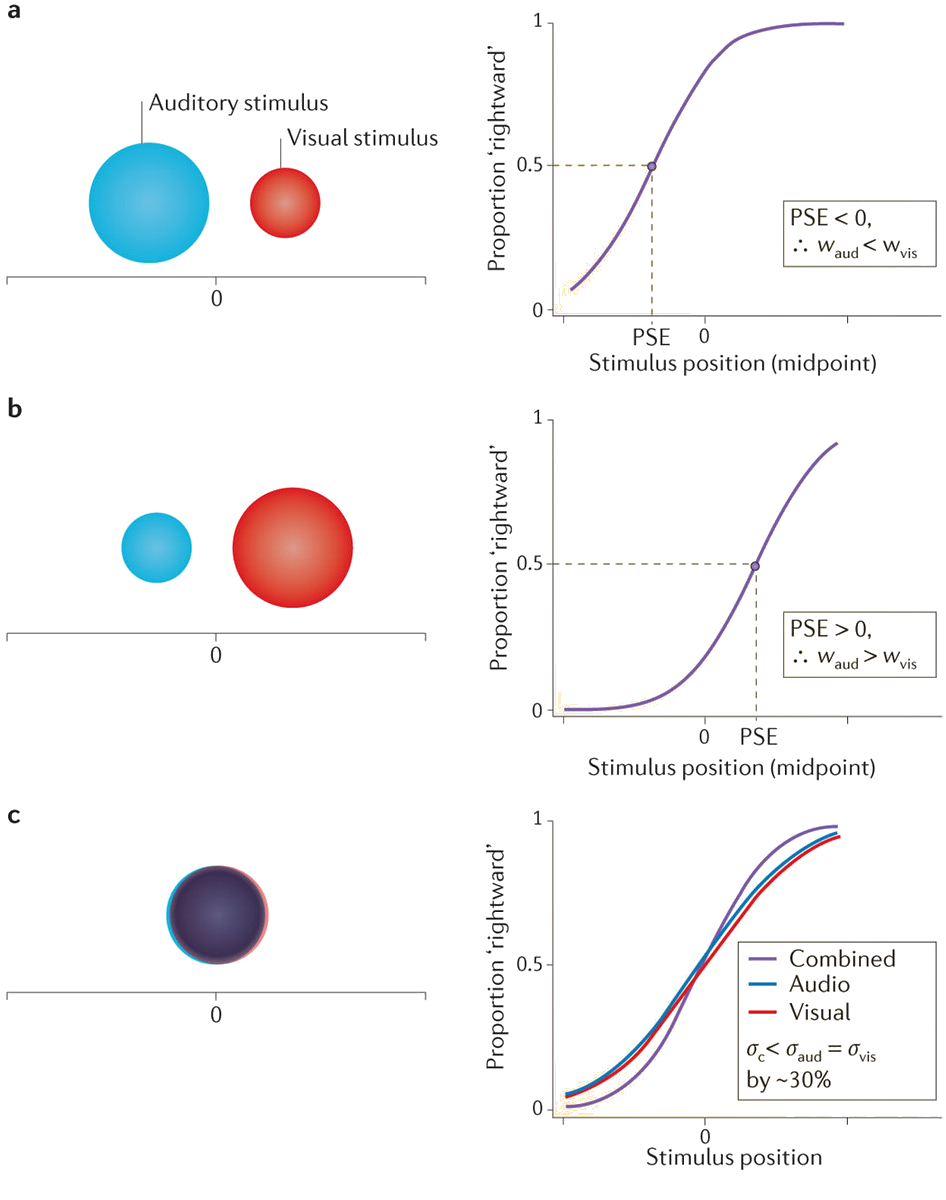
\includegraphics[width=.9\textwidth]{fetsch-visaudloc}
  \caption{Behavioral experiments of visual and auditory localization task. (from \cite{fetsch_bridging_2013})}
  \label{fig:visaudloc}
\end{figure}

Alais and Burr \cite{alais_ventriloquist_2004} used experiments to test human performance in spatial localization tasks (Figure \ref{fig:visaudloc}. In the experiments, subjects were given visual and auditory stimuli and asked to report whether the stimuli were from left or right. Both visual and auditory stimuli were controlled in position and reliability.

In the first experiment (Figure \ref{fig:visaudloc}a), the two modalities of stimuli were in conflict position, where the visual stimulus was displaced on the left. Also the visual stimulus was more reliable (depicted by smaller circle) than the auditory stimulus. With the midpoint of the stimuli changed from left to right, the proportion of subjects choosing right increased from 0 to 1. As shown in the figure, the point of subjective equality (PSE), where subjects have equal tendency of left and right, is smaller than 0. This indicates that the visual cue, which is more reliable, dominates the auditory cue.

In the second experiment (Figure \ref{fig:visaudloc}b), after changing the reliability of the visual stimulus to less than that of the auditory stimulus, the PSE shifted to larger than 0. This also indicates that the more reliable cue is given higher weight, which is in accord with Equation \ref{eq:optweight}.

In the third experiment (Figure \ref{fig:visaudloc}c), the performance of multisensory cue integration was compared against unisensory cue. The visual and auditory stimuli were placed in congruent position with same reliability. The right figure shows that the curve of combined cumulative Gaussian psychometric function has steeper slope than that of unisensory cue. In addition, data show that the standard deviation of combined cue decreased by $30\%$. This is approximate to $1-\sqrt{2}$, which we can calculate using optimal cue integration (Equation \ref{eq:optweight} and \ref{eq:optrel}).

The result indicates that humans perform near-optimally in multisensory perception. It is interesting to note that humans have the ability to adapt to the changing of reliability of cues (by modifying the weight in Equation \ref{eq:optest}). Additionally, experiments also shows that non-human primates have the similar performance in vision-vestibular integration \cite{gu_neural_2008}.

\section{Neurophysiology of Multisensory Integration}
In parallel to psychophysical studies, neuroscientists try to explain multisensory integration phenomena on account of the neural basis.
They use neurophysiological recording or brain imaging to examine the physiological properties of a neuron or a population of neurons that underlies the integration functions.

%As was mentioned in the introduction, the object of neurophysiological study is the neuronal responses (firing rates) of multisensory neurons. The neuronal responses are tested in different conditions of multisensory versus unisensory, 

Multisensory neurons are found in many brain areas, including superior colliculus \cite{stein_merging_1993} and cortex (posterior parietal area \cite{graziano_system_2001} and superior temporal area \cite{alais_multisensory_2010}).
Among all neurophysiological studies, there are two groups of influential work -- the classical multisensory studies in cat superior colliculus (SC) \cite{stein_merging_1993, stein_multisensory_2008} and a recent body of work on vision-vestibular integration in primate dorsal medial superior temporal area (MSTd) \cite{morgan_multisensory_2008, fetsch_visualvestibular_2010}.
In the former studies, some key principles of sensory integration are established. The later studies focus on its mathematical rules and linking the physiological evidence to behavioral observations.

%Researchers found that multisensory neurons are particularly abundant in the superior colliculus (SC), a midbrain structure primarily involved in orienting the eyes and head towards salient stimuli \cite{sparks_translation_1986}. Another area in brain that caught interest from researchers is the dorsal medial superior temporal area (MSTd), which is responsible for integration visual and vestibular cues for detecting self-motion \cite{gu_visual_2006}.

\subsection{Multisensory Integration in SC and Empirical Principles}
The superior colliculus (SC), a structure common to all mammalian brains, is involved in audio-visual and visual-somatosensory integration at a fairly low level. It is ideal for examining properties of multisensory integration because of its low-levelness and multimodal inputs \cite{alais_multisensory_2010}.
By studying the cat SC area for multisensory integration, researchers found a number of empirical principles, which state the properties of multisensory integration \cite{stein_merging_1993}. The most prominent principles are the principle of ``inverse effectiveness'' and the ``spatial/temporal principle''.

Enhancement of multisensory response to spatially congruent stimuli is a basic property for multisensory neurons. However, the effect of the enhancement is found to decrease with increasing stimulus intensity, which is known as ``inverse effectiveness'' \cite{meredith_visual_1986}. More specifically, for spatially congruent stimuli, when the input is weak, the multisensory response may exceed the sum of unisensory responses (superadditivity). As the stimulus intensity increases, the enhancement becomes less salient and the multisensory response tends to be equal or less than the sum of unisensory responses (these cases are termed additivity and subadditivity respectively).

Researchers also have found out the robust enhancement of multisensory response occurs only when the input stimuli are spatially congruent and temporally synchronous \cite{meredith_determinants_1987, meredith_spatial_1996}. When, contrastingly, the inputs are placed in large spatial or temporal disparity, response suppression occurs. This is referred as ``spatial/temporal principle''.

\subsection{Multisensory Integration in Area MSTd}
Although the aforementioned classical empirical principles summarize the key properties of multisensory response, these properties are not described quantitatively. The mathematical combination rule employed by multisensory neurons remains to be found. A comprehensive research on visual-vestibular integration in primate MSTd area has derived a linear combination rule, which closely matches the observation \cite{morgan_multisensory_2008}.

The medial superior temporal area (MSTd) is believed to be involved in visual-vestibular interaction for perceiving self-motion (heading). Different from previous studies, Morgan \etal has probed a broad range of stimulus space and recorded responses in this area \cite{morgan_multisensory_2008}. The data are sufficient for them to characterize the mathematical properties of the multisensory combining rule.

\begin{figure}[tpb]
  \centering
  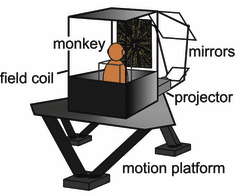
\includegraphics[scale=.6]{apparatus}
  \caption{Apparatus used to study visual-vestibular cue integration. (from \cite{fetsch_visualvestibular_2010})}
  \label{fig:apparatus}
\end{figure}

A ``virtual reality'' motion platform (Figure \ref{fig:apparatus}) is used to control the visual and vestibular stimuli of the study. 
This platform can translate in any horizontal direction to invoke the vestibular stimulus of the monkey seated in the apparatus. Meanwhile, the monkey looks at the moving particles (optical flow) in the screen and receives the visual stimulus of self-motion. The optical flow is controlled to vary in direction and coherence.

During the experiment, a variety of conditions are tested. Conditions include presenting visual cue alone in eight directions, vestibular cue alone in eight directions and 64 ($8 \times 8$) combinations of cues, both congruent and conflicting. The optical flow coherence (visual cue reliability) is manipulated in $100\%$, $50\%$ and $25\%$. Responses of one of the MSTd cells is shown in Figure \ref{fig:coherence}.

\begin{figure}[btp]
  \centering
  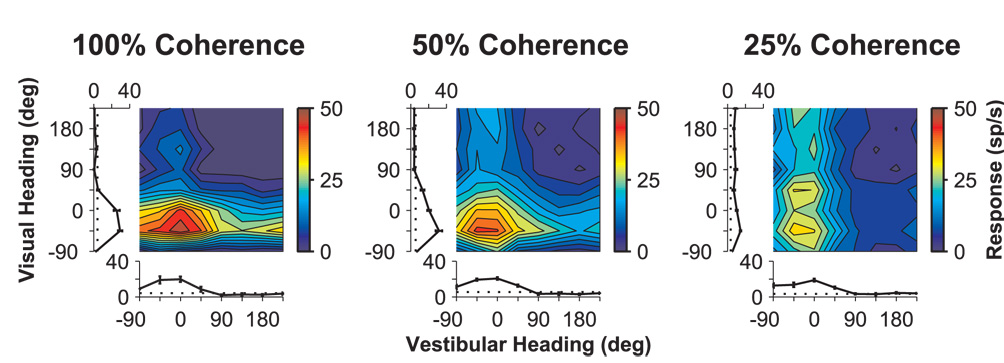
\includegraphics[width=\textwidth]{coherence}
  \caption{Responses of a MSTd cell to multisensory stimulus. Curves along bottom and left margin show the responses when visual and vestibular inputs present alone. The color contour plots show the multisensory response. The visual dominance of heading perception is weakened as optical flow coherence decrease. (from \cite{morgan_multisensory_2008})}
  \label{fig:coherence}
\end{figure}

Morgan \etal tried to address an arithmetic expression that describes the response to multisensory stimulus combinations ($R_{comb}$) as a function of the responses to vestibular and visual stimuli ($R_{vest}$ and $R_{vis}$, respectively) presented separately. A linear combination rule is found to match closely the observed data:
\begin{equation}
  R_{comb}(\phi_{vest}, \phi_{vis}) = w_{vest} R_{vest}(\phi_{vest}) + w_{vis} R_{vis}(\phi_{vis}) + C 
  \label{eq:lincomb}
\end{equation}

In contrast to classical study in SC, which emphasizes superadditivity \cite{meredith_visual_1986}, Morgan \etal found that most MSTd neurons have subadditive responses (\eg $w_{vest} + w_{vis} < 1$). To explain this inconsistency, there are two factors should be taken into account. First, these two studies observed different brain areas. Additionally, other studies also suggest that the superadditivity is far less common in cortex than in SC \cite{alais_multisensory_2010}. Second, the superadditivity is found only if the input stimuli are weak (near the threshold of eliciting a response). However, it is more common that input stimuli are above the threshold and additivity occurs \cite{stanford_evaluating_2005}.

Another interesting finding is that the mixing weights, $w_{vest}$ and $w_{vis}$, depend on the cue reliability (Figure \ref{fig:weight}), which is analogous to psychophysical study of optimal cue integration.
This is neuronal evidence of the ability of animals to adapt to cue reliability changes .

\begin{figure}[tpb]
  \centering
  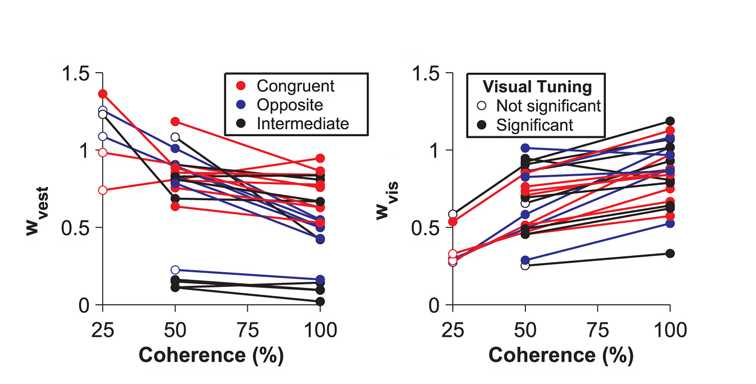
\includegraphics[width=.7\textwidth]{weight}
  \caption{Mixing weights change with optical flow coherence. In most neurons, $w_{vis}$ increases and $w_{vest}$ decreases with coherence.(from \cite{morgan_multisensory_2008})}
  \label{fig:weight}
\end{figure}

%\subsection{Development of multisensory integration}
%Besides understanding the usage of multisensory integration, plentiful of researches are into knowing how multisensory integration is acquired. 

\section{Neural Network Models}
So far, we have mentioned three seemingly isolated studies of multisensory integration -- the psychophysical study of optimal cue integration, the classical empirical principles of multisensory integration in SC and the recent neurophysiological findings in MSTd area. Now, we present two neural network models that bridge the gaps among these studies.

\subsection{The Probabilistic Population Codes for Bayesian Inference}
A number of bio-inspired computational models have been established to account for SC responses and their dependence on cortical input \cite{patton_modeling_2003, alvarado_neural_2008}. These models have successfully showed the computational properties underlying a single multisensory neuron. However, they fail to link the neuronal responses to behavior. A recent theory of probabilistic population codes (PPCs) showed that a population of neurons can apply Bayesian computation and achieve optimal cue integration \cite{ma_bayesian_2006}.

The idea of the model is that using a population of neurons, a sensory cue with Gaussian noise can be encoded by the population response and Bayesian inference can be done by simply taking the linear weighted sum of both unisensory response under certain condition (Poisson-like variability of neuron response).

Consider the response (firing rates) of a population of neurons, $\mathbf{r} = \{ r_1, r_2, \dots, r_N \}$, to a stimulus, $s$. The firing rate of each neuron, $r_i$, has a Poisson distribution with the mean of $f_i(s)$, 
\begin{equation}
  p(r_i|s) = \frac{e^{-f_i(s)} f_i(s)^{r_i}}{r_i!}
  \label{eq:poisson}
\end{equation}
where $f_i$ is the tuning curve of the $i$-th neuron. The tuning curves have the same shape but differ in preferred stimulus. We can simply assume all neurons are uncorrelated, hence
\begin{equation}
  p(\mathbf{r}|s) = \prod_{i} p(r_i|s) = \prod_{i} \frac{e^{-f_i(s)} f_i(s)^{r_i}}{r_i!}
  \label{eq:popvar}
\end{equation}
With this equation, we know, when the stimulus is $s$, what the population activity $\mathbf{r}$ might be. However, actually the observer knows little about $s$. What we are interested in is how to decode $s$ from $\mathbf{r}$.

\begin{figure}[tpb]
  \centering
  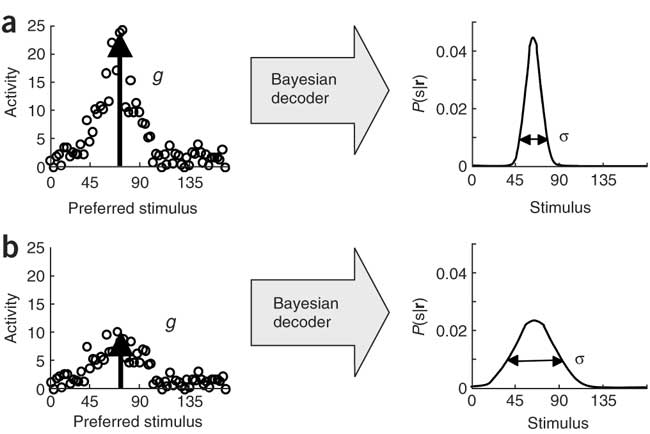
\includegraphics[width=.8\textwidth]{decoder}
  \caption{The mean and variance can be decoded using Bayesian decoder. (from \cite{ma_bayesian_2006})}
  \label{fig:decoder}
\end{figure}

Bayesian decoder is used to find out the mean and variance of $s$, when fixing $\mathbf{r}$ (Figure \ref{fig:decoder}). By Bayes' Rule, the posterior distribution is
\begin{equation}
  p(s|\mathbf{r}) = \frac{p(\mathbf{r}|s)p(s)}{p(\mathbf{r})} \propto p(\mathbf{r}|s)
  \label{eq:posterior}
\end{equation}
Here we assume a flat prior. The best mean of the posterior distribution can be estimated by the peak in the population activity. And the variance is inversely proportional to the amplitude of the peak (the gain).

Now we consider a multisensory integration task. $\mathbf{r}_1$ and $\mathbf{r}_2$ encode the input sensory cues $(c_1, \sigma_1)$ and $(c_1, \sigma_2)$ respectively. These two populations have the same tuning curve profile for individual cell, that is the means of $r_{1i}$ and $r_{2i}$ are both proportional to $f_i(s)$. Simply add up the two population activities, we can get a third population activity, $\mathbf{r}_3 = \mathbf{r}_1 + \mathbf{r}_2$, that encodes the posterior distribution in condition of both cues, \eg $p(s|\mathbf{r}_3) = p(s|\mathbf{r}_1,\mathbf{r}_2)$. By decoding $\mathbf{r}_3$, we can derive the optimal estimate of combined cue and the gain is consistent with Equation \ref{eq:optrel} (Figure \ref{fig:infer}).

\begin{figure}[tpb]
  \centering
  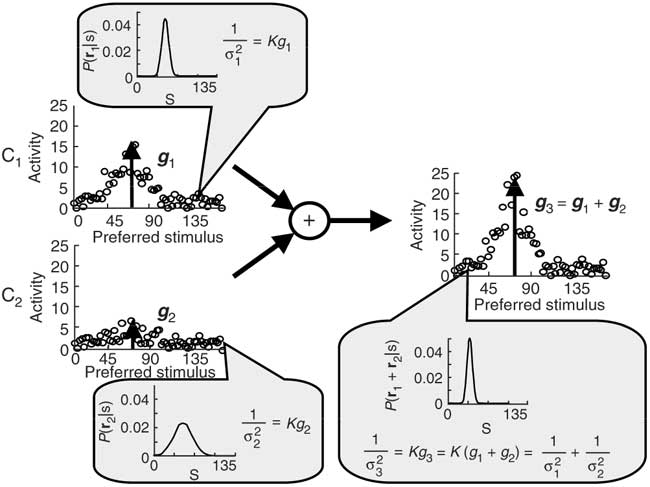
\includegraphics[width=.8\textwidth]{infer}
  \caption{Bayesian inference using probabilistic population codes. (from \cite{ma_bayesian_2006})}
  \label{fig:infer}
\end{figure}

Further study shows that Bayesian inference can also be implemented by PPCs, when the neuron activity has Poisson-like distribution (Poisson-like variability), which is close to observations, or the prior is not flat.

It's important to note that, PPCs gives an explanation of how neuronal responses can be interpreted to behavior. Furthermore, the behavior is consistent with the normative prediction of psychophysics.

\subsection{The normalization model}
Considering a computational model for neuronal response to multisensory stimuli, it is hard to relate the model further to behavior without taking a population of neurons into account. Thus, the normalization model \cite{ohshiro_normalization_2011} for a population of neurons is of particular interest. Surprisingly, this model also helps to explain several key empirical findings: the reliability-dependent combination rule in area MSTd as well as the empirical principles that were initially described in classic studies of the SC.

\begin{figure}[tpb]
  \centering
  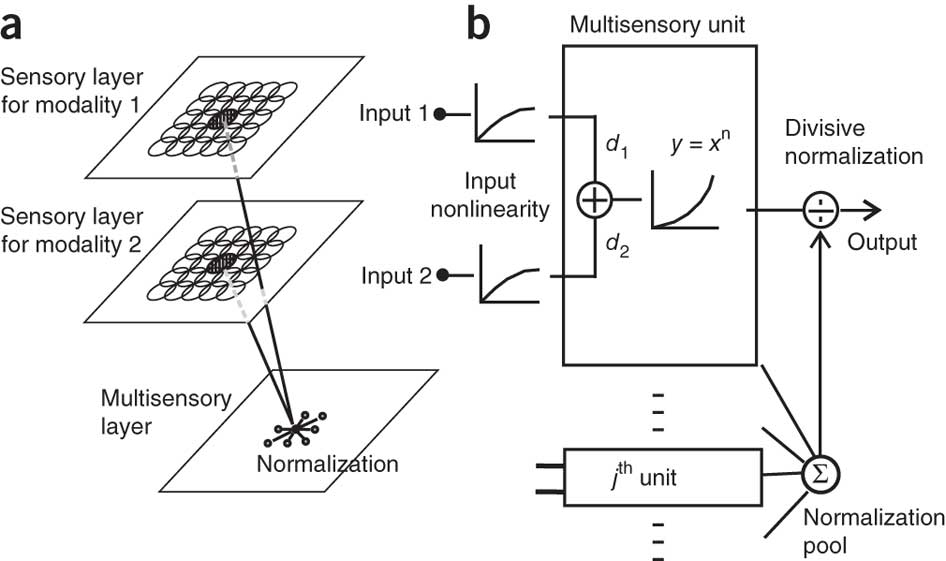
\includegraphics[width=.8\textwidth]{normalize}
  \caption{Schematic illustration of the normalization model. (from \cite{ohshiro_normalization_2011})}
  \label{fig:normalize}
\end{figure}

As shown in Figure \ref{fig:normalize}a, this neural network model has a similar structure as in the two middle levels in Figure \ref{fig:flow}. It consists of two unimodal layers and a multisensory layer. These layers are topographically aligned, which means each multisensory neuron is connected by a pair of unisensory neurons with spatially overlapping receptive fields. The calculation of multisensory output is in two steps (Figure \ref{fig:normalize}). First, each multisensory neuron take the linear weighted sum of unisensory inputs:
\begin{equation}
  E = d_1 I_1(s) + d_1 I_2(s)
  \label{eq:step1}
\end{equation}
where $d_1$ and $d_2$ are termed modality dominance weights. $I_1(s)$ and $I_2(s)$ are the unisensory inputs of stimulus $s$. The second step is normalizing the linear weighted sum over the whole population activity. The final response of a single neuron is
\begin{equation}
  R = \frac{E^n}{\alpha^n+\frac{1}{N}\sum_{j=1}^N E_j^n}
  \label{eq:step2}
\end{equation}
Here the divisive normalization is found commonly existed in many brain areas \cite{carandini_normalization_2012}.

Simulation of the network shows that it can account for the principle of the ``inverse effectiveness'' (Figure \ref{fig:inverse}) and the ``spatial principle'' (Figure \ref{fig:spatial}). 

\begin{figure}[tpb]
  \centering
  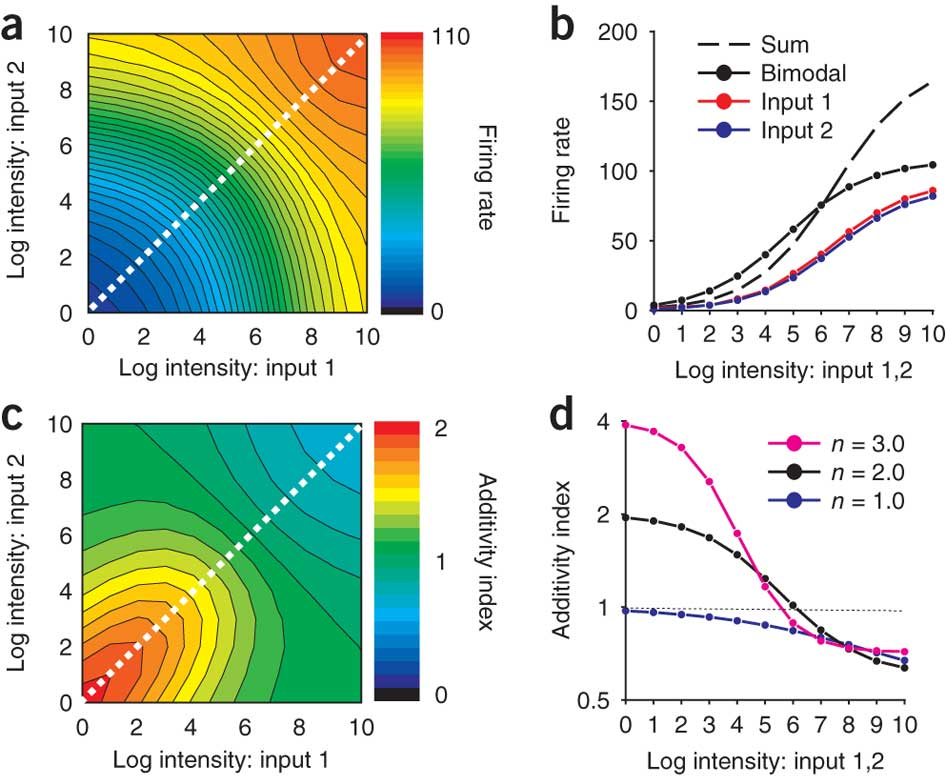
\includegraphics[width=.6\textwidth]{inverse2}
  \caption{The normalization model accounts for the principle of the ``inverse effectiveness''. (from \cite{ohshiro_normalization_2011})}
  \label{fig:inverse}
\end{figure}

    Figure \ref{fig:inverse}a shows the bimodal response as a function of two unisensory responses. Figure \ref{fig:inverse}b is taken from the diagonal of Figure \ref{fig:inverse}a. This plot clearly shows that the bimodal response exceeds the sum of unisensory responses, when the input intensity is low. However, the bimodal response becomes less than the sum as intensity increases.
    Figure \ref{fig:inverse}c,d shows the additivity index \footnote{the ratio of the bimodal response to the sum of unimodal responses} of results from \ref{fig:inverse}a,b.

\begin{figure}[tpb]
  \centering
  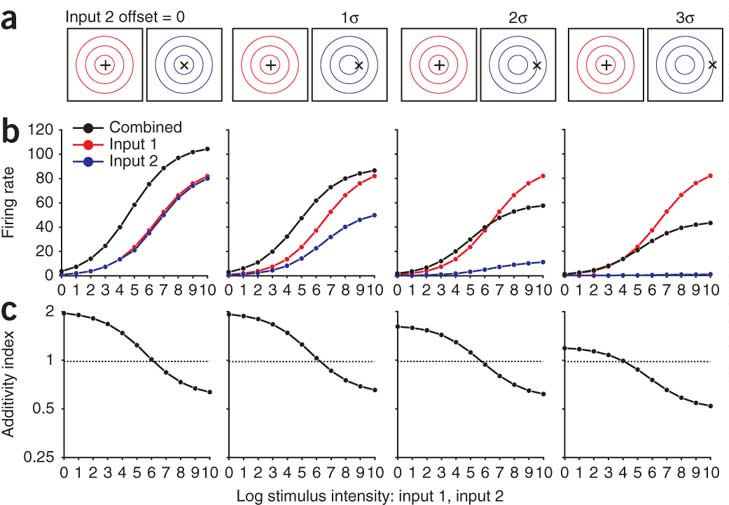
\includegraphics[width=.8\textwidth]{spatial2}
  \caption{The normalization model accounts for the ``spatial principle''. (from \cite{ohshiro_normalization_2011})}
  \label{fig:spatial}
\end{figure}

Figure \ref{fig:spatial}a shows the topological position of the stimuli. The input of the first modality is fixed at the center of the receptive field. The input of the second modality is displaced in away from the center. We can see that, as the offset increases, the multisensory enhancement gets weaker (Figure \ref{fig:spatial}b,c).

\begin{figure}[tpb]
  \centering
  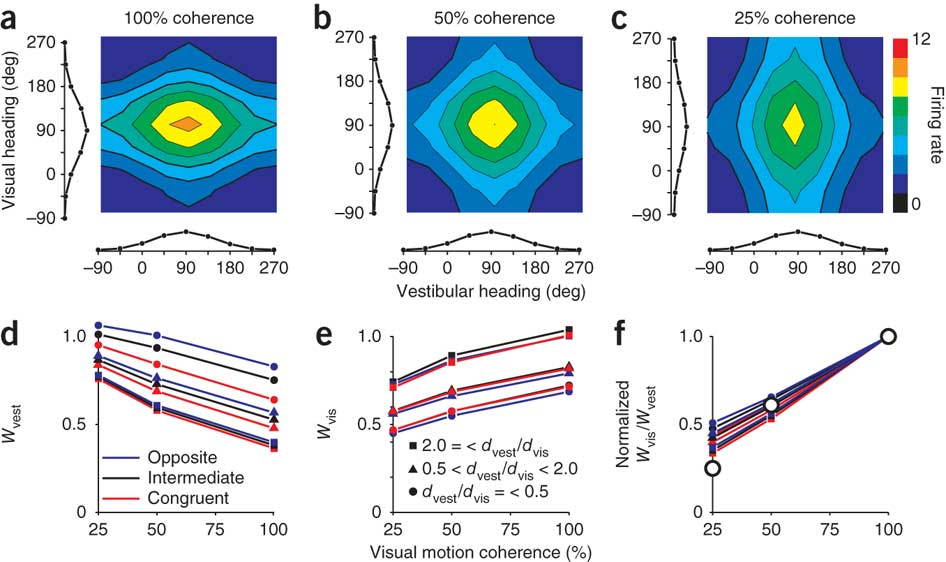
\includegraphics[width=.8\textwidth]{normweight}
  \caption{The normalization model accounts for the linear combination rule which depends on cue reliability. (from \cite{ohshiro_normalization_2011})}
  \label{fig:normweight}
\end{figure}

Notably, the response of the normalization model is also consistent with the linear combination rule predicted in the MSTd area (Equation \ref{eq:lincomb}). The simulation result is shown in Figure \ref{fig:normweight}, which is similar to that in Figure \ref{fig:weight}.

\section{Discussion}
This paper has reviewed the classical and recent findings of the study on understanding multisensory integration in biological systems as well as two neural network models that both give a mathematical description of this process. 

We introduced the linear observer model for maximum reliability which is frequently used in the psychophysical study of multisensory integration. Additionally, this normative prediction is found to match the behavioral prediction in human and other primates.

We also reviewed two groups of influential work in the neurophysiological study of multisensory integration. One is the empirical principles found in cat SC, which describe the properties of response of multisensory neurons. The other one is the reliability-dependent linear combination rule found in primate area MSTd, which describes the underlying computational mechanism of multisensory integration.

At the end, two neural network models are reviewed. The PPCs is the first model that links neuronal response to behavior. The normalization model is at network level and unifies the neurophysiological findings.

Different from other work, both models describe a biological plausible computation method. In other words, Poisson-like variability and normalization operation are both commonly found in brain areas.

Interestingly, these two models focus on accounting for different observations, and a potential combination of these models will be favorable. However, there are still conflicts between these models. PPCs assumes the combination weights are fixed. On the contrary, the mixing weights in the normalization model may vary with the cue reliability. Also, the output of the normalization model cannot be used directly by the PPCs as the latter requires the input to be encoded naturally. Further study is required to resolved the conflicting findings.

\addcontentsline{toc}{section}{References}
\bibliography{bib}
\bibliographystyle{unsrt}

\end{document}
